\section{幂函数、指数函数、对数函数}
\begin{definition}
同一个数\(a\ (a\in\mathbb{R})\)连续相乘\(b\ (b\in\mathbb{N})\)次所得的乘积称作“\(a\)的\(b\)次方”(或“\(a\)的\(b\)次幂”),记作\(a^b\),即\[
a^b = \underbrace{a \times a \times \dotsm \times a}_{b\text{次}} = \prod_{i=1}^b a.
\]

特别地,规定:\(a^0 = 1\),\(a^{-n} = \frac{1}{a^n}\),其中\(a\in\mathbb{R}^*\),\(n\in\mathbb{N}^+\).
\end{definition}

\begin{figure}[ht]
\centering
\begin{tikzpicture}
\def\r{\textcolor{orange}}
\def\b{\textcolor{blue}}
\def\p{\textcolor{purple}}
\draw (0,0)node{\(\r{a}^{\b{b}} = \p{c} \iff \log_{\r{a}} \p{c} = \b{b}\)};
\draw (-2.2,-.5)node{\r{底数}}
	(-2.2,.5)node{\b{指数}}
	(-1,-.5)node{\p{幂}}
	(.3,-.5)node{\r{底数}}
	(1.4,-.5)node{\p{真数}}
	(2.3,.5)node{\b{对数}};
\draw[->] (-1.7,-.3)--(-1.7,-1)--(.84,-1)->(.84,-.3); %a
\draw[->] (-1.55,.3)--(-1.55,1)--(1.7,1)->(1.7,.3); %b
\draw[->] (-.86,.3)--(-.86,.7)--(1.1,.7)->(1.1,.3); %c
\end{tikzpicture}
\caption{底数、指数、幂与对数的联系}\label{figure:函数.底数、指数、幂与对数的联系}
\end{figure}

\subsection{幂函数的概念}
\begin{definition}[幂函数]
函数\(f(x)=x^{\mu}\ (\mu \in \mathbb{R})\),称为\DefineConcept{幂函数}.
\end{definition}

\subsection{幂函数的性质}
\begin{property}
幂函数具有以下性质:
\begin{itemize}
	\item 当\(\mu = 0\)时,幂函数\(f(x)=x^{\mu}\)在定义域\((-\infty,+\infty)\)上恒为一,是常数函数.

	\item 当\(\mu\)为正奇数时,幂函数\(f(x)=x^{\mu}\)为奇函数,
	其定义域、值域均为\((-\infty,+\infty)\),它在定义域内恒单调递增.

	\item 当\(\mu\)为正偶数时,幂函数\(f(x)=x^{\mu}\)为偶函数,
	其定义域为\((-\infty,+\infty)\),其值域为\([0,+\infty)\),
	它在\((-\infty,0]\)上单调递减,在\([0,+\infty)\)上单调递增.

	\item 当\(\mu\)为负奇数时,幂级数\(y=x^{\mu}\)又称为\DefineConcept{比例函数},
	其定义域、值域为\((-\infty,0)\cup(0,+\infty)\),
	它在区间\((-\infty,0)\)和\((0,+\infty)\)内单调递减.

	若幂函数前有常系数大于零则称之为\DefineConcept{正比例函数}.
	% Mathematica: Plot[Evaluate[x^-n /. n -> {1, 2, 3, 4, 5}], {x, 0, 2}, PlotRange -> {0, 2}, PlotLegends -> Automatic]

	若幂函数前有常系数小于零则称之为\DefineConcept{反比例函数}.
	% Mathematica: Plot[Evaluate[x^-n /. n -> {1, 2, 3, 4, 5}], {x, -2, 0}, PlotRange -> {-2, 2}, PlotLegends -> Automatic]

	\item 当\(\mu\)为负偶数时,幂函数\(f(x)=x^{\mu}\)为偶函数,
	其定义域为\((-\infty,0)\cup(0,+\infty)\),其值域为\((0,+\infty)\),
	它在\((-\infty,0)\)内单调递增,在\((0,+\infty)\)内单调递减.

	\item 当\(\mu = \pm\frac{m}{n} \in \mathbb{Q}\)(\(m,n>0\)且\(m\)、\(n\)是互质的整数)时,
	幂函数\(f(x)=x^{\mu}=x^{\pm\frac{m}{n}}\)可改写为\(y=\sqrt[n]{x^m}\)(\(\mu>0\)时)
	或\(y=\frac{1}{\sqrt[n]{x^m}}\)(\(\mu<0\)时).
\end{itemize}
\end{property}

\begin{figure}[ht]
	\centering
	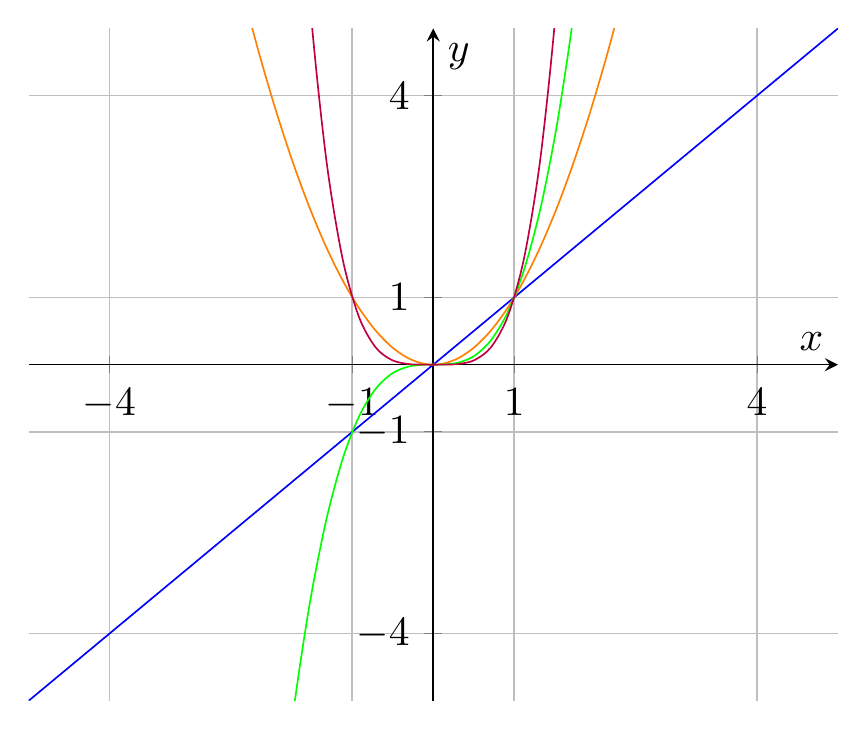
\begin{tikzpicture}[scale=1.5]
		\begin{axis}[
			xmin=-5,xmax=5,
			ymin=-5,ymax=5,
			enlargelimits,
			axis lines=middle,
			xlabel=$x$,
			ylabel=$y$,
			xtick={-4,-1,1,4},
			ytick={-4,-1,1,4},
			grid=major,
		]
			\begin{scope}[samples=50,smooth,domain=-5:5]
				\addplot[color=blue]{x};
				\addplot[color=orange]{x^2};
				\addplot[color=green]{x^3};
				\addplot[color=purple]{x^4};
			\end{scope}
		\end{axis}
	\end{tikzpicture}
	\caption{}
\end{figure}

\begin{figure}
	\centering
	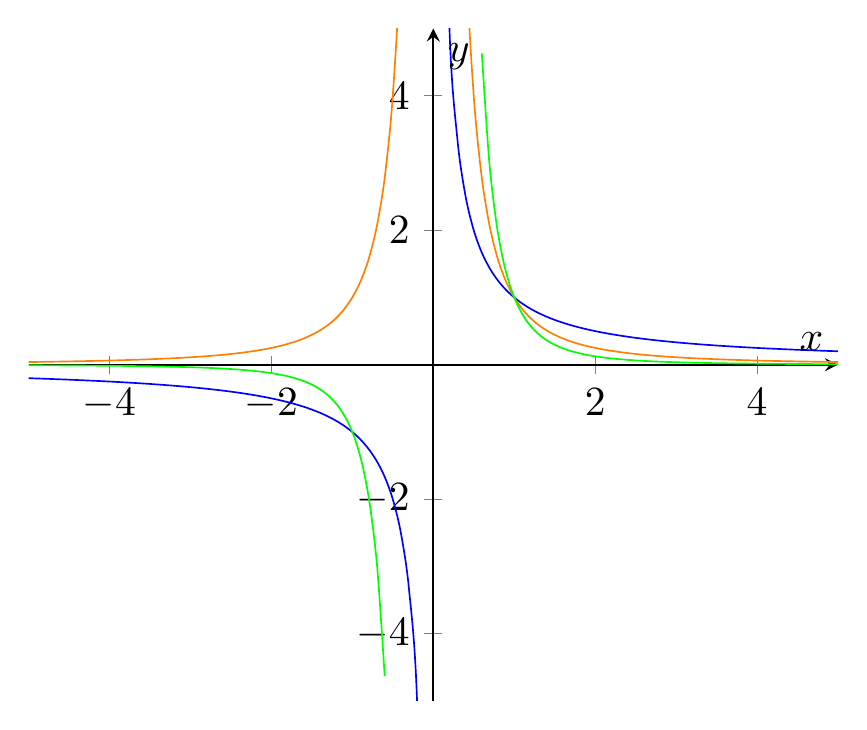
\begin{tikzpicture}[scale=1.5]
		\begin{axis}[
			xmin=-5,xmax=5,
			ymin=-5,ymax=5,
			enlargelimits,
			axis lines=middle,
			xlabel=$x$,
			ylabel=$y$,
		]
			\begin{scope}[samples=50,smooth]
				\begin{scope}[domain=-5:-.1]
					\addplot[color=blue]{1/x};
					\addplot[color=orange]{1/(x^2)};
					\addplot[color=green,domain=-5:-.6]{1/(x^3)};
				\end{scope}
				\begin{scope}[domain=.1:5]
					\addplot[color=blue]{1/x};
					\addplot[color=orange]{1/(x^2)};
					\addplot[color=green,domain=.6:5]{1/(x^3)};
				\end{scope}
			\end{scope}
		\end{axis}
	\end{tikzpicture}
	\caption{}
\end{figure}

\subsection{指数函数的概念}
\begin{definition}[指数函数]
形如\(y=a^x\ (a>0 \land a \neq 1)\)的函数,称为以\(a\)为底的\DefineConcept{指数函数}.
将\(a\ (a \neq 0)\)的倒数\(\frac{1}{a}\)记作\(a^{-1}\).
将\(a\ (a \geq 0)\)的\(x\)次方根\(\sqrt[x]{a}\)记作\(a^{\frac{1}{x}}\).
规定任一实数的1次幂为该实数本身,即\(a^1=a\).
规定任一非零实数的零次幂为1,即\(a^0=1\).
\end{definition}

\subsection{对数函数的概念}
\begin{definition}[对数函数]
形如\(y=\log_a x\ (a>0 \land a \neq 1)\)的函数,称为以\(a\)为底的\DefineConcept{对数函数}.

特别地,以\(10\)为底的对数称为\DefineConcept{常用对数},记作\(y = \lg x\);
以常数\(e\)为底的对数称为\DefineConcept{自然对数},记作\(y = \ln x\).
\end{definition}

\subsection{指数函数、对数函数的性质}
\begin{property}
指数函数\(y = a^x\)与对数函数\(y = \log_a x\)互为反函数,即\[
	a^{\log_a x} = x, \qquad
	\log_a a^x = x.
\]
它们具有以下性质:
\begin{gather}
	a^x a^y = a^{x+y}, \\
	\log_a xy = \log_a x + \log_a y, \\
	\frac{a^x}{a^y} = a^{x-y}, \\
	\log_a \frac{x}{y} = \log_a x - \log_a y, \\
	(a^x)^y = a^{xy}, \\
	\log_a x^y = y \log_a x.
\end{gather}
\end{property}

\begin{theorem}[换底公式]
一般地,\[
\log_a b = \frac{\log_c b}{\log_c a},
\]其中\(a,c\in(0,1)\cup(1,+\infty)\),\(b\in(0,+\infty)\).

特殊地,\[
\log_a b = \frac{1}{\log_b a},
\]其中\(a,b\in(0,1)\cup(1,+\infty)\).
\end{theorem}

\begin{corollary}
若\(a,a^x \in (0,1)\cup(1,+\infty)\),则\[
\log_{a^x} b^y = \frac{y}{x} \log_a b.
\]
\end{corollary}

\begin{example}
证明:\begin{equation}\label{equation:函数.真底互换公式}
a^{\ln b} = b^{\ln a}.
\end{equation}
\begin{proof}
在\cref{equation:函数.真底互换公式} 等号左右变量分别取对数,得\[
\ln(a^{\ln b}) = \ln b \ln a, \qquad
\ln(b^{\ln a}) = \ln a \ln b,
\]显然两者相等,故\(a^{\ln b} = b^{\ln a}\)成立.
\end{proof}
\end{example}

\subsection{重幂}
设\(a\)是实数,\(b\)是正整数,定义:\[
	\relax^ba \defeq \underbrace{a^{a^{\iddots^a}}}_{\text{\(b\)个}},
\]
我们把\(\relax^ba\)读作“\(a\)的\(b\) \DefineConcept{重幂}”.

例如,\[
	\relax^23 = 3^3, \qquad
	\relax^33 = 3^{3^3}, \qquad
	\relax^43 = 3^{3^{3^3}}.
\]
